\scanpage{104}
\mspage{103}%
tions sur $F$ (décroissantes, \inserted{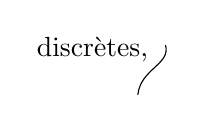
\begin{tikzpicture}[baseline=-.2ex,x=1em,y=1em]
\node[anchor=base west] at (0,.55) {discrète\handwritten{s,}};
\draw (5,.95) .. controls (5.2,.25) and (4.1,.1) .. (4,-.85);
\end{tikzpicture}} indexées par $\underline{Z}$) compatibles avec lesproduits tensoriels (en utilisant la notion év\deleted{\unsure{o|q}}\handwritten{i}dente de produ\rlap{q}it tensoriel\deleted{s} de deux espaces vectoriels fi\rlap{g}l\rlap{l}trés). On notera qu\deleted{e}'une telle donnée ne pourra plus s'exprimer par un homomorphisme d'un certain groupe algébrique dans $G$ (le groupe de Galois de $\underline{C}$ en $F$), car la catégorie des espaces vect\rlap{r}o\rlap{o}riels de dimension finie sur $k$, munis d'une\rlap{\tikz[baseline=0pt,x=1em,y=1em]{\draw (.05,.8)--(.08,.96);}} filtration décroissante discrète indexée par $\underline{Z}$, n'est pas une catégorie abélienne\rlap{\tikz[baseline=0pt,x=1em,y=1em]{\draw (0,-.55)--(.05,-.7);\fill (-.04,-.85) circle (.045);}} (les bimorphismes ne sont pas des isomorphismes\handwritten{!}). Mais à une telle donnée est associée un deuxiè\deleted{e}me foncteur fibre\margin{\handwritten{$F'$}} $\inserted{\unsure{F|\mathbb{F}}'(V)=}\rlap{\handwritten{\tikz[baseline=0pt,x=1em,y=1em]{\draw (.35,.4) .. controls (.7,-.25) and (-3.5,-.2) .. (-3.6,-.6) .. controls (-3.8,-.8) and (-3.75,-1.1) .. (-3.6,-1.15);}}}\operatorname{Gr}F(V)$, à valeurs cette fois-ci dans les vectoriels gradués (NB $F$ joue le rôle de la cohomologie de \deleted{Hodge, $F'$} De Rham, $F'$ cel\rlap{l}u\rlap{e}i de la cohomologie de Hodge\deleted{\unsure{)}}, muni de la graduation \deleted{totale}\inserted{\handwritten{par $p$}}). La donnée de $F'$ correspond alors à un torseur \inserted{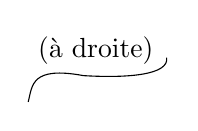
\begin{tikzpicture}[baseline=-.2ex,x=1em,y=1em]
\node[anchor=base west] at (0,.5) {\handwritten{(à droite)}};
\draw (5,.5) .. controls (5.1,-.1) and (3.7,-.25) .. (2,-.15) .. controls (.1,.2) and (.15,-.5) .. (0,-1.1);
\end{tikzpicture}} $P$ sous $G$, le groupe de Galois correspondant $G'$ étant déduit de $G$ en tordant par $P$. La graduation de $F'$ correspond à un homomorphisme $i_{\handwritten{1}}:\underline{G}_m\handwritten{\longrightarrow}G'$. Considérons alors sur $F'$ la filtration décroissante associée à sa gra\unsure{\rlap{u}d|d}\rlap{d}uation, et soit $H'_{i_{\handwritten{1}}}=\underline{\operatorname{Aut}}\,\underline{\mathrm{filt}}^{\handwritten{!}}(F')\handwritten{\subset}\underline{\operatorname{Aut}}(F')=G'$ le sous-schéma en groupes de $G$ qui correspond aux \inserted{$\otimes$-}\rlap{\handwritten{\tikz[baseline=0pt,x=1em,y=1em]{\draw (-.9,.2) .. controls (-.4,.05) and (-.1,-.7) .. (-.2,-.8) .. controls (-.5,-.7) and (.1,-.2) .. (.7,.3);}}}automorphismes de $F'$ (ou plutôt des $F'_{k'}$, $k'$ une $k$-algèbre quelconque) qui respectent sa filtration\inserted{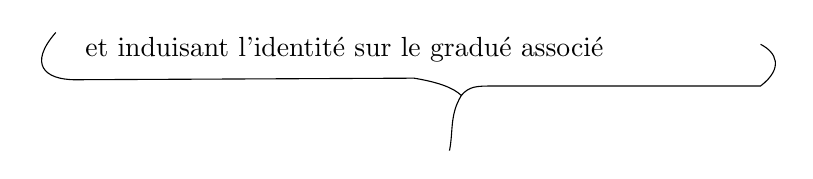
\begin{tikzpicture}[baseline=-.2ex,x=1cm,y=1cm]
\node[anchor=base west] at (0,.3) {\handwritten{et induisant l'identité sur le gradué associé}};
\draw (-.25,.6) .. controls (-.6,.2) and (-.4,0) .. (0,0) -- (4.3,.02) .. controls (4.6,-.03) and (4.8,-.1) .. (4.9,-.2) .. controls (5,-.08) and (5.1,-.08) .. (5.3,-.08) -- (8.7,-.08) .. controls (9,.15) and (8.9,.35) .. (8.7,.45);
\draw (4.9,-.2) .. controls (4.75,-.45) and (4.8,-.65) .. (4.75,-.9);
\end{tikzpicture}}; il est canoniquement déterminé par $i_{\handwritten{1}}$. On peut aussi regarder le sous-schéma
\[
Q=\underline{\operatorname{Isom}}\,\underline{\mathrm{filt}}^{\handwritten{!}}(F,F')\handwritten{\subset}P=\underline{\operatorname{Isom}}(F,F')
\]
du schéma $P$ des $\otimes$-isomorphismes de $F$ avec $F'$, \deleted{formé de} qui correspond aux \rlap{i}a\rlap{s}u\rlap{t}omorphismes respectant les filtrations de $F$ et $F'$\inserted{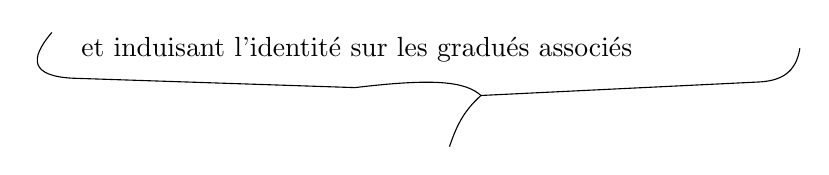
\begin{tikzpicture}[baseline=-.2ex,x=1cm,y=1cm]
\node[anchor=base west] at (0,.3) {\handwritten{et induisant l'identité sur les gradués associés}};
\draw (-.25,.6) .. controls (-.55,.25) and (-.5,.05) .. (0,.02) -- (3.6,-.1) .. controls (4.6,.02) and (5,-.02) .. (5.2,-.2) -- (8.7,-.03) .. controls (9,-.02) and (9.2,.08) .. (9.25,.4);
\draw (5.2,-.2) .. controls (5,-.38) and (4.9,-.55) .. (4.8,-.85);
\end{tikzpicture}}. C'est à priori un pseudo-torseur à \deleted{droite}\inserted{\handwritten{gauche}} sous $H'$, \rlap{\tikz[baseline=0pt,x=1em,y=1em]{\draw (.15,.25) .. controls (.2,0) and (.1,-.2) .. (.17,-.5);}}i.e. il est vide ou un torseur à droite sous $H'$. \uuline{Il faudrait prouver} que c'est bien un torseur (i.e. que sur une extension convenable $k'$ de $k$, on peut \rlap{y}trouver un isomorphisme\margin{\handwritten{\tikz[baseline=0pt,x=1em,y=1em]{\draw (0,0)--(.15,.18);}}} de $F_{k'}$ avec $F'_{k'}$ \uline{respectant les filtrations}). Donc on trouve une restriction d\rlap{e}u groupe d'opérateurs (à \deleted{droite}\inserted{\handwritten{gauche}}) $G'$ de $P$ au sous-groupe $H'$,

